\chapter{模型与两个估计目标}
\label{chap:model}

第二章的综述把研究缺口归结为两点：当期再生数之外的估计目标缺少误差分析，环境方差缺少一把折算成病例数的尺子。本章建立一个包含环境层、负二项传播与二项报告的单代模型，在四条明确假设下推导两个估计目标的有限样本方差。第~\ref{sec:model-setup}~节给出模型与报告病例数的精确分布；第~\ref{sec:model-targets}~节定义两个估计目标并列出基本假设；第~\ref{sec:model-current}~节讨论当期再生数的估计；第~\ref{sec:model-average}~节推导跨期平均水平的方差并定义交叉点；第~\ref{sec:model-reporting}~节比较报告率与覆盖面两条扩容途径。各命题的完整证明放在附录~A，正文给出推导思路与直觉。

\section{传播与报告的两层模型}
\label{sec:model-setup}

\subsection{模型设定}

考虑第 $t$ 期的传播。上一代有 $n$ 名感染者，第 $i$ 人产生 $X_{i,t}$ 个继发感染。为刻画超传播，设给定当期再生数 $R_t$ 时 $X_{i,t}$ 相互独立，服从负二项分布
\begin{equation}
  X_{i,t}\mid R_t \sim \NB\Bigl(k,\ \frac{k}{k+R_t}\Bigr),\qquad
  \E(X_{i,t}\mid R_t)=R_t,\quad \Var(X_{i,t}\mid R_t)=R_t+\frac{R_t^2}{k}.
  \label{eq:offspring}
\end{equation}
这里 $k$ 是离散参数。由第~\ref{sec:lit-tools}~节的混合表示，式~\eqref{eq:offspring} 等价于个体再生数服从均值为 $R_t$、形状参数为 $k$ 的 Gamma 分布，继发感染数在其上服从泊松分布\citep{lloydsmith2005superspreading}。方差中的 $R_t$ 是泊松部分，$R_t^2/k$ 是个体传染力差异带来的部分，$k$ 越小这一部分越大。

同期新感染总数 $I_t=\sum_{i=1}^{n}X_{i,t}$。由负二项分布的可加性，$I_t\mid R_t\sim\NB(nk,\,k/(k+R_t))$。监测系统只看到其中一部分，每名新感染者独立地以概率 $\rho$ 被报告，报告病例数 $C_t\mid I_t\sim\Bin(I_t,\rho)$。图~\ref{fig:mechanism} 示意了这一过程：顶部的环境层表示同一期所有感染者共享同一个 $R_t$。左栏的 $n$ 名感染者经负二项传播产生数目差别很大的新感染者，其中一人产生 7 个，体现超传播；右栏的二项抽稀让每名新感染者独立地以概率 $\rho$ 进入监测数据，图中 11 名新感染者里有 3 名被报告。监测系统只能看到最终的报告数 $C_t$，传播与报告两层随机性都包含在其中。

\begin{figure}[!tbp]
  \centering
  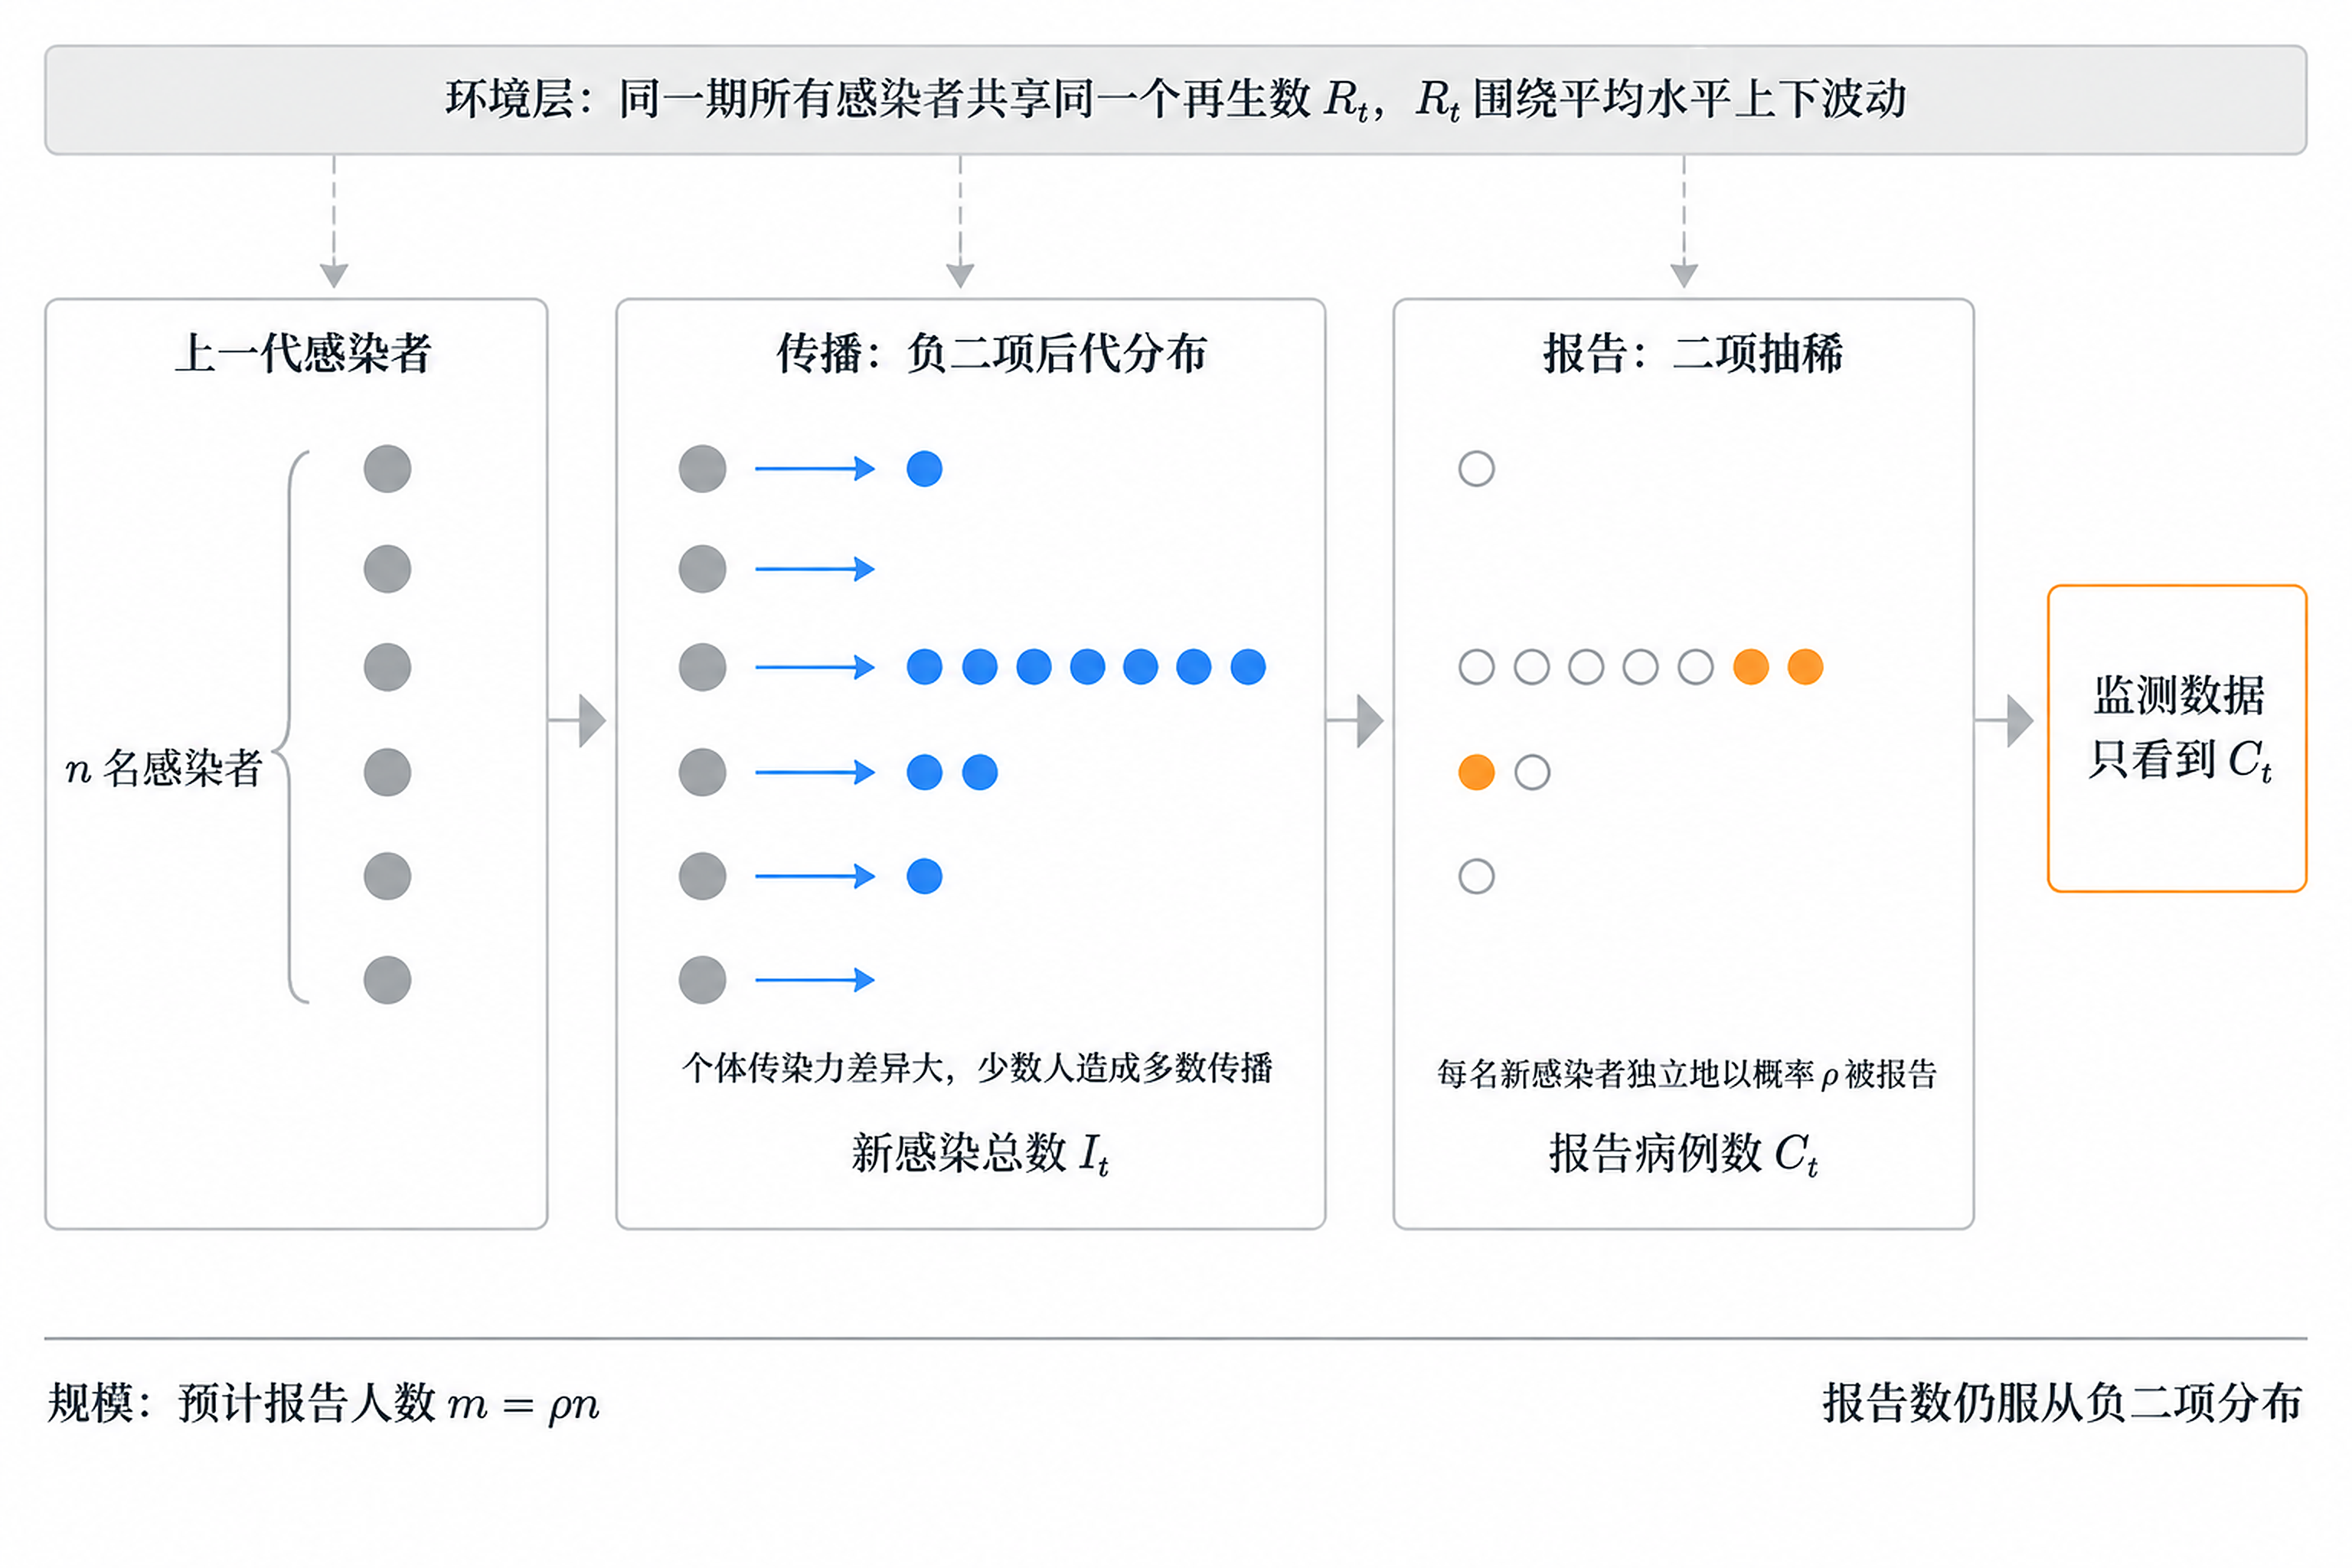
\includegraphics[width=\textwidth]{figures/fig_3_1_mechanism.png}
  \caption{传播与报告的两层模型示意。环境层决定当期再生数 $R_t$，上一代 $n$ 名感染者按负二项后代分布产生新感染者，新感染者再经二项抽稀成为报告病例；监测数据只记录报告病例数 $C_t$。}
  \label{fig:mechanism}
\end{figure}

\subsection{报告病例数的精确分布}

由第~\ref{sec:lit-tools}~节的抽稀封闭性，把 $I_t$ 的分布代入式~\eqref{eq:thinning-pgf}，得到报告病例数的条件分布
\begin{equation}
  \begin{gathered}
  C_t\mid n, R_t \sim \NB\Bigl(nk,\ \frac{k}{k+\rho R_t}\Bigr),\\
  \E(C_t\mid n,R_t)=\rho n R_t,\qquad
  \Var(C_t\mid n,R_t)=\rho n R_t+\frac{\rho^2 n R_t^2}{k}.
  \end{gathered}
  \label{eq:report-dist}
\end{equation}
推导只需一步。$I_t$ 的概率生成函数为 $\{k/(k+R_t-R_t s)\}^{nk}$，以 $1-\rho+\rho s$ 代 $s$，分母变为 $k+\rho R_t-\rho R_t s$，形状参数 $nk$ 不变，$R_t$ 被替换为 $\rho R_t$。所以报告过程相当于把再生数打了一个 $\rho$ 折扣，分布族不变。

记 $m=\rho n$，即上一代感染者中预计被报告的人数，下文用 $m$ 度量监测规模。$m$ 同时依赖覆盖的感染者人数 $n$ 和报告率 $\rho$。在住院监测中，$n$ 可以理解为辖区内上一代的全部感染者，$\rho$ 为感染者中住院并被记录的比例，$m$ 则近似等于上一周的报告住院数。

报告数的相对方差可以写成两项之和：
\begin{equation}
  \frac{\Var(C_t\mid n,R_t)}{\E(C_t\mid n,R_t)^2}=\frac{1}{\rho n R_t}+\frac{1}{nk}.
  \label{eq:relvar}
\end{equation}
第一项来自报告抽样，与预计报告数 $\rho nR_t$ 成反比，提高报告率可以压低它；第二项来自超传播，只与感染者人数 $n$ 和离散参数 $k$ 有关，与报告率无关。报告率再高，第二项也不会消失，因为它描述的是传播本身的随机性，与观测是否完整无关。这一不对称在第~\ref{sec:model-reporting}~节会以命题的形式再次出现。

\section{两个估计目标与基本假设}
\label{sec:model-targets}

\subsection{估计目标的区分}

$R_t$ 随时间波动。天气、学校假期和人群流动让各期的传播强度围绕某个平均水平上下变化，第二章列举的湿度与城市化证据\citep{shaman2010absolute, dalziel2018urbanization}说明这种波动有实在的来源。设 $\E(R_t)=\Rbar$，$\Var(R_t)=v_R$，称 $v_R$ 为环境方差。

监测要回答的问题可以分为两类。目标Ⅰ是当期再生数 $R_t$。例如卫生部门想知道本周的传播是否比上周更快，或者某项干预实施后传播是否减弱，关心的是这一期实际发生的 $R_t$。目标Ⅱ是平均水平 $\Rbar$。例如为一个流行季制定床位计划，或比较不同季节的典型传播强度，需要的是该时段有代表性的传播水平，单期的 $R_t$ 只是围绕 $\Rbar$ 的一次随机实现。

两个目标使用同一个估计量 $\widehat R_t=C_t/(\rho n)$，误差的参照对象不同。目标Ⅰ的误差是 $\widehat R_t-R_t$，目标Ⅱ的误差是
\begin{equation}
  \widehat R_t-\Rbar=(\widehat R_t-R_t)+(R_t-\Rbar).
  \label{eq:error-split}
\end{equation}
右端第一项是测量误差，随规模缩小；第二项是环境偏离，与规模无关。目标Ⅱ因此比目标Ⅰ多出一个不随规模变化的误差来源。这一分解是全章的出发点，后面的命题都是对它的定量刻画。

\subsection{基本假设}

本章与第四章的推导依赖以下四条假设。

\begin{enumerate}[label=H\arabic*]
  \item 给定 $R_t$，各感染者的继发感染数相互独立且服从式~\eqref{eq:offspring}，报告过程为独立二项抽样。
  \item 同一期的感染者共享同一个 $R_t$，即环境扰动作用在“期”这一层面。
  \item 离散参数 $k$ 与报告率 $\rho$ 已知。
  \item 规模 $n$ 与当期环境无关：$\E(R_t\mid n)=\Rbar$，$\Var(R_t\mid n)=v_R$。
\end{enumerate}

H1 是分支过程的标准假设，在流行早期易感者耗竭可以忽略时较为合理。它排除了感染者之间的相互影响，例如同一家庭内多名感染者共同传播给同一个人。H2 把环境波动放在期的层面，同一期内所有感染者面对同一个传播强度。若同一期内不同亚群面对不同环境，H2 可以放宽为多个环境的汇总，见第~\ref{sec:model-pooling}~节。

H3 在实践中只是近似。$k$ 需要从接触追踪或暴发规模数据中估计\citep{lloydsmith2005superspreading, endo2020estimating}，$\rho$ 需要从血清学调查或负担估计中推算\citep{reed2009estimates, tokars2018seasonal}。$k$ 与 $\rho$ 未知时，估计量的形式不变，方差中会多出参数不确定性的贡献，第四章讨论增长检验时会说明 $k$ 设定偏差的影响。

H4 需要单独说明。若 $n$ 由设计固定，例如每期追踪固定数目的指示病例，H4 自然成立。若 $n_t$ 是此前传播的结果，而 $R_t$ 又有时间相关，那么大的 $n_t$ 往往出现在 $R$ 偏高的时期，H4 不再自动成立。真实监测序列属于后一种情况，规模本身是随机的，第~\ref{sec:design-renewal}~节专门用更新过程的模拟讨论随机规模的影响。

本章其余部分使用的主要符号汇总于表~\ref{tab:symbols}。

\begin{table}[!tbp]
  \centering
  \caption{主要符号}
  \label{tab:symbols}
  \small
  \begin{tabularx}{\textwidth}{@{}lX@{}}
    \toprule
    符号 & 含义 \\
    \midrule
    $R_t$ & 第 $t$ 期的当期再生数，目标Ⅰ \\
    $\Rbar$，$v_R$ & 当期再生数的跨期平均水平与环境方差，$\Rbar$ 为目标Ⅱ \\
    $k$ & 负二项后代分布的离散参数，越小表示超传播越明显 \\
    $n$ & 上一代感染者人数 \\
    $\rho$ & 每名新感染者被报告的概率 \\
    $m=\rho n$ & 预计报告规模，即上一代感染者中预计被报告的人数 \\
    $I_t$，$C_t$ & 第 $t$ 期新感染总数与报告病例数 \\
    $\widehat R_t=C_t/(\rho n)$ & 两个目标共用的估计量 \\
    $A=\Rbar+\rho(\Rbar^2+v_R)/k$ & 规模项系数 \\
    $V(m)=v_R+A/m$ & 目标Ⅱ的估计方差 \\
    $\mx=A/v_R$ & 交叉点，规模项与环境项相等时的预计报告规模 \\
    $\mathcal{I}(R_t)$ & 报告病例数关于 $R_t$ 的 Fisher 信息 \\
    \bottomrule
  \end{tabularx}
\end{table}

\section{当期再生数的估计}
\label{sec:model-current}

先看目标Ⅰ。此时 $R_t$ 视为固定参数，估计量的性质由式~\eqref{eq:report-dist} 直接决定。

\begin{proposition}[当期再生数的有效估计]
\label{prop:current}
在 H1--H3 下，给定 $n$ 与 $R_t>0$，估计量 $\widehat R_t=C_t/(\rho n)$ 满足：
\begin{enumerate}[label=(\roman*)]
  \item $\widehat R_t$ 是 $R_t$ 的极大似然估计；当 $C_t=0$ 时，似然在边界 $R_t=0$ 处取最大值；
  \item $\widehat R_t$ 无偏，方差为 $\Var(\widehat R_t\mid n,R_t)=R_t/(\rho n)+R_t^2/(kn)$；
  \item 对任意 $n$，该方差都等于 Cramér--Rao 下界 $1/\mathcal I(R_t)$，其中 $\mathcal I(R_t)=n/(R_t/\rho+R_t^2/k)$；
  \item $\widehat R_t$ 是 $R_t$ 的一致最小方差无偏估计。
\end{enumerate}
\end{proposition}

推导的核心是把对数似然对 $R_t$ 求导。略去与 $R_t$ 无关的常数，由式~\eqref{eq:nb-pmf} 与式~\eqref{eq:report-dist}，对数似然为
\begin{equation}
  \ell(R_t)=C_t\log R_t-(nk+C_t)\log(k+\rho R_t).
  \label{eq:loglik}
\end{equation}
对 $R_t$ 求导并通分，分子中含 $C_t\rho R_t$ 的两项相互抵消，得到
\begin{equation}
  S(R_t)=\frac{C_t}{R_t}-\frac{\rho(nk+C_t)}{k+\rho R_t}
  =\frac{k\,(C_t-\rho nR_t)}{R_t(k+\rho R_t)}
  =\mathcal{I}(R_t)\,(\widehat R_t-R_t),
  \label{eq:score}
\end{equation}
其中 $\mathcal{I}(R_t)=k\rho n/[R_t(k+\rho R_t)]=n/(R_t/\rho+R_t^2/k)$。四条结论都可以从这个式子读出。令 $S=0$ 得到 $\widehat R_t$，这是结论 (i)；若 $C_t=0$，$\ell(R_t)=-nk\log(k+\rho R_t)$ 在 $R_t\ge0$ 上单调递减，最大值落在边界 0。由式~\eqref{eq:report-dist}，$\E\widehat R_t=R_t$，方差为 $\Var(C_t)/(\rho n)^2$，化简即得结论 (ii)。得分函数恰好是估计误差的 $\mathcal{I}(R_t)$ 倍，满足第~\ref{sec:lit-tools}~节所述 Cramér--Rao 等号成立的条件，因此方差等于 $1/\mathcal{I}(R_t)$，这是结论 (iii)。

结论 (iii) 不是渐近结果。通常极大似然估计只在样本量趋于无穷时才渐近达到下界，这里在每个有限 $n$ 处都精确达到。原因是负二项分布在 $k$ 已知时是以 $C_t$ 为充分统计量的单参数指数族，而 $\widehat R_t$ 恰好是充分统计量的线性函数。结论 (iv) 来自同一事实，即 $C_t$ 是完备充分统计量，$\widehat R_t$ 是它的无偏函数，由 Lehmann--Scheff\'e 定理即为一致最小方差无偏估计\citep{lehmann1998point, casella2002statistical}。精确达到下界需要 $k$ 已知；$k$ 未知时，模型变为两参数，$C_t$ 不再是完备充分统计量。

方差的两部分与式~\eqref{eq:relvar} 一一对应，$R_t/(\rho n)$ 来自报告抽样，$R_t^2/(kn)$ 来自超传播。两部分都按 $1/n$ 衰减，规模越大，当期再生数估得越准，没有底板。Parag 等在泊松更新模型下发现信息与病例数成正比\citep{parag2022quantifying}，命题~\ref{prop:current} 是信息正比于病例数在负二项与漏报下的精确形式，在 $k\to\infty$ 且 $\rho=1$ 时，$\mathcal{I}(R_t)=n/R_t$，回到泊松情形。超传播使信息打了折扣，$k$ 越小折扣越大。

为核对结论 (iii)，在 $m$ 从 1 到 1000 的 10 个规模上各做 20,000 次模拟，方差与 Cramér--Rao 下界之比在 0.98--1.02，差异在蒙特卡洛误差范围内（图~\ref{fig:variance}a 中的圆点）。

\section{跨期平均水平与交叉点}
\label{sec:model-average}

\subsection{方差结构}

目标Ⅱ要估计的是 $\Rbar$。此时 $R_t$ 是随机的，估计误差多出了式~\eqref{eq:error-split} 中的环境偏离项。

\begin{proposition}[跨期平均水平的方差]
\label{prop:average}
在 H1--H4 下，$\widehat R_t=C_t/(\rho n)$ 是 $\Rbar$ 的无偏估计，其方差为
\begin{equation}
  V(m)=\Var(\widehat R_t\mid n)=v_R+\frac{\Rbar}{\rho n}+\frac{\Rbar^2+v_R}{kn}
  =v_R+\frac{A}{m},\qquad A=\Rbar+\frac{\rho(\Rbar^2+v_R)}{k}.
  \label{eq:var-average}
\end{equation}
定义交叉点 $\mx=A/v_R$，则：
\begin{enumerate}[label=(\roman*)]
  \item $m\to\infty$ 时 $V(m)\to v_R$；
  \item 规模项在总方差中的份额为 $1/(1+m/\mx)$，在 $m=\mx$ 处两项各占一半；
  \item 规模从 $m$ 翻倍到 $2m$，方差下降的比例为 $1/[2(1+m/\mx)]$；
  \item $V(m)$ 严格递减且严格凸，对 $m$ 的弹性为 $-\mx/(m+\mx)$，在 $m=\mx$ 处等于 $-1/2$。
\end{enumerate}
\end{proposition}

式~\eqref{eq:var-average} 由全方差公式~\eqref{eq:total-variance} 得到，取条件变量为 $R_t$。由 H4，条件于 $n$ 时 $R_t$ 的均值与方差仍为 $\Rbar$ 与 $v_R$。条件均值 $\E(\widehat R_t\mid R_t)=R_t$，它的方差就是环境方差 $v_R$；条件方差由命题~\ref{prop:current}(ii) 给出，对 $R_t$ 取期望时，$R_t$ 的一次项变为 $\Rbar$，二次项变为 $\E(R_t^2)=\Rbar^2+v_R$，于是得到 $\Rbar/(\rho n)+(\Rbar^2+v_R)/(kn)$。把 $n=m/\rho$ 代入，两项合并为 $A/m$。$A$ 中出现 $\Rbar^2+v_R$ 而非 $\Rbar^2$，是因为超传播项与 $R_t$ 的平方成正比，环境波动让平方的期望变大。

四条结论都是 $V(m)=v_R+A/m$ 的初等推论。规模项份额为 $(A/m)/(v_R+A/m)$，分子分母同除以 $A/m$ 即得 $1/(1+m/\mx)$。翻倍降幅为 $[V(m)-V(2m)]/V(m)=(A/2m)/(v_R+A/m)$，正是份额的一半。弹性为 $V'(m)\,m/V(m)=-(A/m)/(v_R+A/m)$，即份额的相反数。二阶导数 $V''(m)=2A/m^3>0$，所以 $V$ 严格凸。这几个量的共同点是都只依赖比值 $m/\mx$：交叉点把不同参数下的方差曲线统一到同一把尺子上，规模达到交叉点的几倍，就可以直接读出规模项还剩多少份额、翻倍还能降多少。

\subsection{交叉点的含义与数值示例}

交叉点的含义要说清楚。$V(m)$ 处处凸，曲线上没有拐点，也没有斜率突然变化的位置，所以 $\mx$ 不是收益突然消失的阈值。它的作用是给规模提供一把尺子。规模低于 $\mx$ 时，误差主要来自病例太少，扩大规模收效明显；规模高于 $\mx$ 时，误差主要来自环境波动，翻倍的收益迅速变小。从 $\mx=A/v_R$ 的形式看，环境越稳定（$v_R$ 越小），交叉点越大，需要更多病例才能让环境项成为主要误差；超传播越明显（$k$ 越小）或报告率越高，$A$ 越大，交叉点也越大。

图~\ref{fig:variance} 用一组示例参数画出这一结构，取 $\Rbar=1.15$，$v_R=0.04$，$k=0.35$，$\rho=0.25$。此时 $A=2.1232$，$\mx=53.1$。左图在双对数坐标下比较两个目标的方差。目标Ⅰ的方差取 $R_t=\Rbar$ 时的 Cramér--Rao 下界，是一条斜率为 $-1$ 的直线，规模每扩大 10 倍方差就降为十分之一。目标Ⅱ的方差在小规模时与目标Ⅰ几乎重合，过了交叉点后逐渐向水平虚线 $v_R$ 靠拢，在 $m=1000$ 附近已经很难与底板区分。两条曲线在小规模处重合的原因是此时规模项远大于 $v_R$，环境偏离被测量误差淹没；在大规模处分离，则是因为测量误差已经被压到环境偏离之下。空心点为每个规模 20,000 次模拟的方差，两个目标的模拟值与理论值之比都落在 0.98--1.02。

右图给出环境项占比与翻倍降幅。环境项占比是一条 S 形曲线，在交叉点处为 50\%；翻倍降幅从小规模时接近 50\% 单调下降。规模为 10、53.1 和 200 时，翻倍降幅依次为 42.1\%、25.0\% 和 10.5\%。也就是说，在示例参数下，从 200 例扩大到 400 例，目标Ⅱ的方差只降低约十分之一，同样的扩容对目标Ⅰ却意味着方差减半。规模收益在交叉点前后连续变化，两侧的收益差异来自同一条凸曲线的不同位置。

\begin{figure}[!tbp]
  \centering
  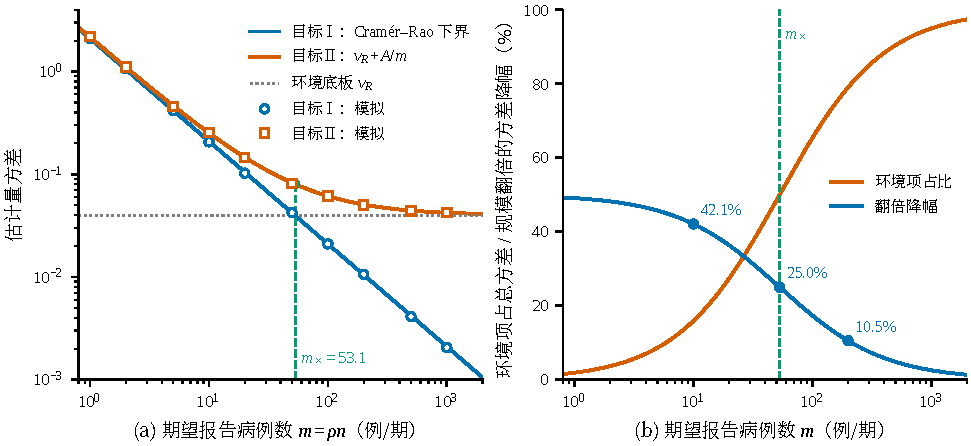
\includegraphics[width=\textwidth]{figures/fig_3_3_variance_theory.pdf}
  \caption{两个估计目标的方差结构。参数为 $\overline{R}=1.15$，$v_R=0.04$，$k=0.35$，$\rho=0.25$，对应 $A=2.1232$，$m_\times=53.1$。（a）目标Ⅰ的方差（取 $R_t=\overline{R}$ 时的 Cramér--Rao 下界）与目标Ⅱ的方差 $v_R+A/m$ 随规模的变化，空心点为每个规模 20,000 次模拟的方差，竖虚线标出交叉点。（b）环境项在目标Ⅱ总方差中的占比与规模翻倍带来的方差降幅，三个标注点对应 $m=10$、$m_\times$ 与 200。}
  \label{fig:variance}
\end{figure}

\subsection{跨环境汇总}
\label{sec:model-pooling}

底板 $v_R$ 在单一环境内无法通过扩大规模消除，但可以通过汇总多个环境来压低。设 $J$ 个辖区的环境方差同为 $v_R$，两两相关系数的平均值为 $\bar c$。等权平均的环境项方差为 $(v_R/J^2)[J+J(J-1)\bar c]$，整理得
\begin{equation}
  v_R\,\bar c+\frac{v_R(1-\bar c)}{J}.
  \label{eq:pooling}
\end{equation}
式~\eqref{eq:pooling} 把底板分成两部分：$v_R\bar c$ 是各辖区共同的环境波动，汇总再多辖区也无法消除；$v_R(1-\bar c)/J$ 是辖区特有的波动，随辖区数增加而下降。各辖区的扰动不完全同步时（$\bar c<1$），汇总能降低底板；完全同步时（$\bar c=1$）汇总无效。这与两阶段抽样中整群内相关决定设计效应的道理相同\citep{kish1965survey}。对流感而言，绝对湿度等气候驱动在相邻地区高度同步\citep{shaman2010absolute}，可以预期 $\bar c$ 不小，汇总能压低的部分有限。第六章用全国加总序列与州级序列的对比估计这一点。

汇总改变的是底板，规模项也会相应变化：汇总后的规模为各辖区规模之和，规模项按总规模缩小。因此跨环境汇总同时作用于两项，交叉点会相应移动，移动方向取决于 $\bar c$ 与辖区数。

\section{报告率与覆盖面}
\label{sec:model-reporting}

\subsection{两条扩容途径的不对称}

$m=\rho n$ 可以通过两条途径扩大，即提高报告率 $\rho$，或扩大覆盖的人群使 $n$ 增大。前者对应提高检测率、改进报告流程，后者对应增加哨点医院、扩大监测辖区。式~\eqref{eq:var-average} 表明两者的作用并不相同。

\begin{proposition}[报告率与覆盖面的不对称]
\label{prop:reporting}
在 H1--H4 下：
\begin{enumerate}[label=(\roman*)]
  \item 固定 $n$ 令 $\rho\to1$，$V\to v_R+\Rbar/n+(\Rbar^2+v_R)/(kn)$，极限严格大于 $v_R$；
  \item 固定 $\rho$ 令 $n\to\infty$，$V\to v_R$；
  \item 报告项可以拆为 $\Rbar/(\rho n)=\Rbar/n+(1-\rho)\Rbar/(\rho n)$，第二部分是漏报带来的额外方差；
  \item 把 $n$ 与 $\rho$ 各提高相同的小比例，前者带来的方差下降是后者的 $A/\Rbar=1+\rho(\Rbar^2+v_R)/(k\Rbar)$ 倍。
\end{enumerate}
\end{proposition}

结论 (i) 与 (ii) 直接由式~\eqref{eq:var-average} 的中间形式得到。$\rho$ 只出现在报告项 $\Rbar/(\rho n)$ 的分母中，超传播项 $(\Rbar^2+v_R)/(kn)$ 不含 $\rho$，所以即使报告完全，超传播项仍然存在。$n$ 同时出现在两项的分母中，扩大覆盖可以把两项都压到零。结论 (iii) 把报告项拆成完整报告时也会存在的部分 $\Rbar/n$ 与漏报带来的额外部分，$\rho=1$ 时后者为零。

结论 (iv) 比较边际效果。对 $\log n$ 求导，两项都按 $1/n$ 变化，方差的变化为 $-A/m$；对 $\log\rho$ 求导，只有报告项变化，方差的变化为 $-\Rbar/m$。两者之比为 $A/\Rbar$。它大于 1，表明在同样的相对增幅下扩大覆盖总是更有效；超出 1 的部分 $\rho(\Rbar^2+v_R)/(k\Rbar)$ 随报告率线性增长，报告率越高、超传播越明显，两条途径的差距越大。

\subsection{不对称的数量大小}

命题~\ref{prop:reporting} 在定性上说明扩大覆盖优于提高报告率，但差距大小取决于 $\rho$。图~\ref{fig:levers} 画出 $A/\Rbar$ 随报告率的变化，横轴为对数刻度，三条曲线对应 $k=0.1$、0.35 和 1，其余参数取示例值。三条曲线都从左侧接近 1 的位置出发，随 $\rho$ 增大而上升，$k$ 越小上升越快。报告完全时（$\rho=1$），三者分别为 12.85、4.39 和 2.18，即在超传播很强的情形下扩大覆盖的边际效果是提高报告率的十余倍。示例参数（$\rho=0.25$，$k=0.35$）对应图中的菱形，$A/\Rbar=1.85$，扩大覆盖的效果接近提高报告率的两倍。$k=0.35$ 时这一比值在 $\rho=0.295$ 处达到 2。

\begin{figure}[!tbp]
  \centering
  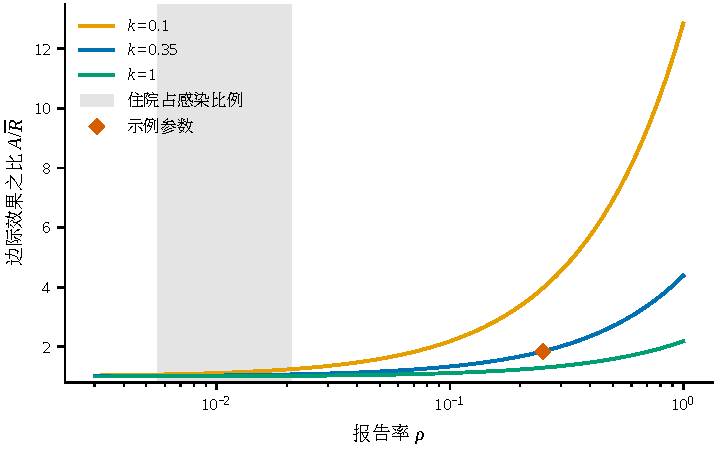
\includegraphics[width=0.72\textwidth]{figures/fig_3_4_levers.pdf}
  \caption{扩大覆盖与提高报告率的边际效果之比 $A/\overline{R}$ 随报告率的变化。$\overline{R}=1.15$，$v_R=0.04$；灰色带为流感住院占感染比例的范围 0.0056--0.021，菱形为示例参数 $\rho=0.25$、$k=0.35$。}
  \label{fig:levers}
\end{figure}

图中灰色带标出流感住院占感染比例的范围，约为 0.0056--0.021\citep{zhou2012hospitalizations, tokars2018seasonal}。在这一范围内三条曲线都贴近 1：$k=0.35$ 时比值为 1.019--1.071。第五章使用的情景参数取 $\Rbar=1.67$、$k\in[0.2,0.5]$，此时这一比值为 1.02--1.18。对住院数据而言，两条途径的边际效果几乎相同，选择哪一条主要看成本。报告率很低时，报告项 $\Rbar/(\rho n)$ 远大于超传播项，方差几乎全部来自报告抽样，提高 $\rho$ 与扩大 $n$ 都在压低同一项。

这一数量判断修正了一个容易产生的误解，即认为超传播使提高报告率在任何情况下都事倍功半。不对称在报告率高、超传播强的情形下才显著，例如接触追踪或暴发调查；在住院、死亡这类报告率很低的监测指标上，两条途径近乎等价。

\section{本章小结}
\label{sec:model-summary}

本章在负二项传播与二项报告的两层模型下，区分了两个估计目标。命题~\ref{prop:current} 表明，对当期再生数，报告病例数除以预计报告规模的估计量在每个有限规模上精确达到 Cramér--Rao 下界，规模收益持续存在，超传播只是让信息打了折扣。命题~\ref{prop:average} 表明，对跨期平均水平，估计方差为环境底板加规模反比项，交叉点 $\mx=A/v_R$ 是两项相等时的规模。规模达到交叉点时再翻一倍只能把方差降低 25\%；曲线处处凸，交叉点是刻度而非阈值。汇总多个环境可以压低底板中辖区特有的部分，共同的环境波动无法通过汇总消除。命题~\ref{prop:reporting} 表明扩大覆盖的边际效果总是不低于提高报告率，两者之比为 $A/\Rbar$，但在住院监测的低报告率下这一比值接近 1。

这些结论依赖 H1--H4，其中 H4 在真实序列中不自动成立。第四章先在 H1--H4 下把方差结构转化为监测设计的定量结论，再用更新过程的模拟考察放宽 H4 后单代公式的适用程度。
